% !TeX root = ../main.tex
\chapter{数学和运动学基础}
\section{空间中位姿的表示}
\subsection{位置的坐标表示}
从本文开始我们就提到SLAM需要解决的一个很重要的问题,那就是系统的位姿如何表述。这里的“位姿”包含了两种含义:一个是“位置”,一个是“姿态”。在一个视觉SLAM系统中,位置的表示还是比较简单的,二维空间用$x,y$两个坐标来描述:
\begin{equation}
	\vec x = [x,y]^T
\end{equation}
相应的,在一个三维空间中用$x,y,z$三个坐标来表示:
\begin{equation}
	\vec x = [x,y,z]^T
\end{equation}
但是在一个SLAM系统中,我们常用射影空间中的齐次坐标来表示点的坐标。齐次坐标的意思就是在原有的坐标上添加一维。在齐次坐标下,空间点可以用一个四维向量来表示:
\begin{equation}
\boldsymbol{x}=\left[x_{1}, x_{2}, x_{3}, w\right]^{T}
\end{equation}
齐次坐标和三维空间点有如下对应关系:
\begin{equation}
	[x,y,z,1]^T=\left[\frac{x_{1}}{w}, \frac{x_{2}}{w}, \frac{x_{3}}{w}, 1\right]^{T}
\end{equation}
从上式可看出,齐次坐标下某个点的每个分量同乘一个非零常数后,仍然表示同一个点,比如$[2,2,4,4]$和$[4,4,8,8]$均表示三维空间中$[0.5,0.5,1]$这个点。空间坐标的表示不用欧几里得坐标,而选择用齐次坐标是有原因的,齐次坐标在运动学计算中有独特的优势\footnote{齐次坐标能够直接与表征位姿的4$\times$4(二维情况下是3$\times$3)矩阵T相乘,大大化简了计算。}。\par

\subsection{二维空间位姿表示}
对于二维空间中的点来说$(x,y)$足以描述一个点的信息。但是对于刚体来说,不但需要位置信息,还需要姿态信息,直观来说就是旋转角度,才能完整的描述刚体的状态。刚体的位姿可以用两个平移量和一个旋转角表示。我们来考虑两个坐标系:局部坐标系O'和世界坐标系O,我们把局部坐标系$O'-X'Y'$下的点$[x_r,y_r]$,转化为世界坐标系$O-XY$下的坐标$[x_w,y_w]$,那么我们可以得到
\begin{figure}
	\centering
	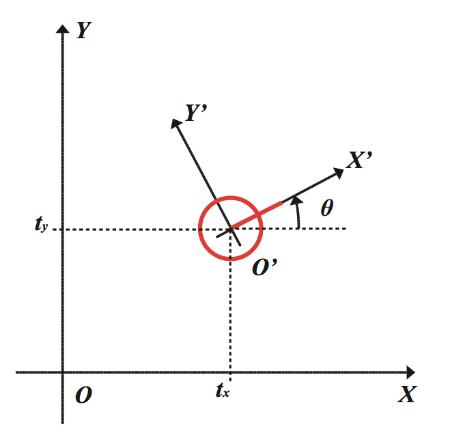
\includegraphics[height=5cm]{figures/2DCoordinate.png}
	\caption{2D坐标系转换}
\end{figure}
\begin{equation}
\left\{\begin{array}{l}{x_{w}=x_{r} \cos \theta-y_{r} \sin \theta+t_{x}} \\ {y_{w}=x_{r} \sin \theta-y_{r} \cos \theta+t_{y}}\end{array}\right.
\end{equation}
我们可以将其写成矩阵形式:
\begin{equation}
\vec{x_{w}}=\vec{R x_{r}}+\vec{t}\label{2dtranslate matrix}
\end{equation}
其中,
\begin{equation}
\mathbf{R}=\left[ \begin{array}{cc}{\cos \theta} & {-\sin \theta} \\ {\sin \theta} & {\cos \theta}\end{array}\right]
\end{equation}
\begin{equation}
\mathbf{t}=\left[t_{x}, t_{y}\right]^{T}
\end{equation}
$\vec R$是一个正交阵,我们称其为旋转矩阵,$\vec t$是平移向量。通过旋转矩阵$\vec{R}$和向量$\vec{t}$,我们准确的描述出局部坐标系的性质。
\subsection{变换矩阵和齐次坐标}
确实,公式\ref{2dtranslate matrix}表达了2D空间的旋转和平移,不过这里还存在一个问题:变换并不是一个线性的变换。假如我们进行了如下两次变换:$\vec R_1,\vec t_1$和$\vec R_2,\vec t_2$,满足:
\begin{equation}
\vec b = \vec R_1 \vec a + \vec t_1,\quad \vec c=\vec R_2 \vec b + \vec t_2
\end{equation}
从$\vec a$到$\vec c$的变换:
\begin{equation}
\vec c=\vec R_2(\vec R_1 \vec a + \vec t_1) + \vec t_2
\end{equation}
可以看到,这样的形式在多次坐标变换之后会变得十分复杂,但我们通过引入齐次坐标,并将变换矩阵重写一下就会发现:
\begin{equation}
\left[ \begin{array}{l}{b} \\ {1}\end{array}\right]=\left[ \begin{array}{ll}{R_{2\times 2}} & {t_{2\times 1}} \\ {0^{T}} & {1}\end{array}\right] \left[ \begin{array}{l}{a} \\ {1}\end{array}\right] = T_{3\times 3} \left[ \begin{array}{l}{a} \\ {1}\end{array}\right]
\end{equation}
我们将a的齐次坐标形式写作 $\vec{\widetilde{a}}$,可得:
\begin{equation}
\vec{\widetilde{c}} =\vec{ T_{cb}T_{ba}}\vec{\widetilde{a}}
\end{equation}
看,齐次坐标能够化简计算难度,通过将一个二维向量末尾添加1,将其变成三维向量,然后将旋转和平移写进同一个矩阵里面,让整个变成一个线性关系。我们称T为\textbf{变换矩阵(Transform Matrix)}。\par
\subsection{三维空间位姿表示}
上面介绍了二维空间的位姿描述,以此类推的话,三维空间的位姿表示也很简单:
\begin{equation}
\boldsymbol{T}=\left[ \begin{array}{ll}{\boldsymbol{R}_{3 \times 3}} & {\boldsymbol{t}_{3 \times 1}} \\ {\mathbf{0}_{1 \times 3}^{T}} & {I_{1 \times 1}}\end{array}\right]
\end{equation}
我们现在有了旋转矩阵来描述旋转,有了变换矩阵来描述一个6自由度的刚体运动,但是请注意,旋转矩阵有9个参数,而旋转只有三个自由度,这样的表达是冗余的;同时变换矩阵有16个参数,而刚体运动只有6个自由度,这样的描述也是冗余的。下面介绍其他几种更紧凑的旋转表示方法。
\subsubsection{欧拉角}
旋转矩阵虽然能够描述旋转,但是非常不直观,人们很难通过这个旋转矩阵想象出这个旋转怎么变换的。而欧拉角提供了一种非常直观的方式来描述旋转,把三维旋转分解成绕不同轴的旋转:偏航角、俯仰角、滚转角。\par
\begin{itemize}
\item 偏航角:绕物体的Z轴旋转
\item 偏航角:绕旋转之后的Y轴旋转
\item 滚转角:绕旋转之后的X轴旋转
\end{itemize}
\begin{figure}[htb]
	\centering
	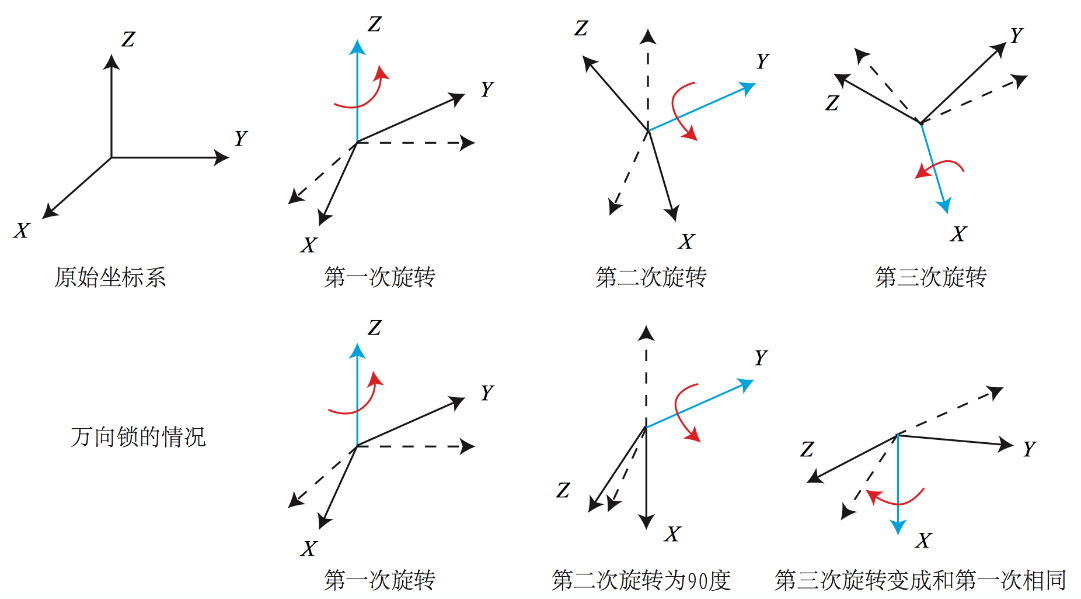
\includegraphics[height=5cm]{figures/GimbalLock.png}
	\caption{万向锁示意图}
\end{figure}\par
因此我们可以用这样一个三维的向量描述任意的旋转,我们能非常直观的想象出旋转的过程。但欧拉角有一个缺陷——万向锁问题(Gimbal Lock):在俯仰角为时,第一次旋转与第三次旋转将变成同一个,这就使得由三维旋转变成了两次旋转,丢失了一个自由度。这被称为奇异性问题,在其他形式的欧拉角中也同样存在。理论上可以证明,只要是通过三个实数来描述三维旋转,就会存在奇异性问题,因此,我们在后面的研究将不会采用欧拉角来表达姿态。
\subsubsection{四元数}
旋转矩阵用9个量描述3个自由度的旋转,具有冗余性;欧拉角和旋转向量是紧凑的,但是具有奇异性。事实上,我们找不到不带奇异性的三维向量表达方式\cite{rotationgroup}。四元数相较于欧拉角不存在万向锁问题,是一种紧凑易于迭代的姿态表示方法,相较于旋转向量,四元数最直观的好处就是省空间,因为一个旋转向量用9个分量来描述,但旋转只有三个自由度,而三个量来描述旋转会遇到奇异性问题,因此我们考虑使用四个量来刻画旋转。
四元数是一种扩展的复数,一个四元数拥有一个实部和三个虚部:
\begin{equation}
q=q_{0}+q_{1} i+q_{2} j+q_{3} k
\end{equation}
其中,i, j, k为四元数的三个虚部,这三个虚部满足以下关系式:
\begin{equation}
\left\{\begin{array}{c}{i^{2}=j^{2}=k^{2}=-1} \\ {i j=k, j i=-k} \\ {j k=i, j k=-i} \\ {k i=j, i k=-j}\end{array}\right.
\end{equation}
我们能用单位四元数表示三维空间中的任意一个旋转,单位四元数是模长为1的四元数。假设某个旋转是绕单位向量$\boldsymbol{n}=\left[n_{x}, n_{y}, n_{z}\right]^{T}
$为轴旋转$\theta$,那么这个旋转用四元数可表示为:
\begin{equation}
\mathbf{q}=\left[\cos \frac{\theta}{2}, n_{x} \sin \frac{\theta}{2}, n_{y} \sin \frac{\theta}{2}, n_{z} \sin \frac{\theta}{2}\right]^{T}
\end{equation}
反之,通过任意单位四元数,可以计算对应的转轴与夹角:
\begin{equation}
\left\{\begin{array}{c}{\theta=2 \cos ^{-1} q_{0}} \\ {\left[n_{x}, n_{y}, n_{z}\right]^{T}=\frac{\left[q_{1}, q_{2}, q_{3}\right]^{T}}{\sin \frac{\theta}{2}}}\end{array}\right.
\end{equation}
\subsubsection{旋转向量}
我们知道,任何一个旋转都可以用一个\textbf{转轴}和一个\textbf{旋转角}来刻画。可以设想这么一个向量,它的方向和旋转轴的方向一致,它的长度和旋转角度的大小一致,我们称这样的向量为\textbf{旋转向量(Axis-Angle)}。这种方法只需要三个量就能表示旋转,再加上表示位置的平移向量,正好6个参数表达一个6自由度的位姿变换。\par
那么剩下的问题是,旋转向量和旋转矩阵是如何转换的呢?旋转向量并不能直接用来计算,它只是旋转的一种表示方法,具体的计算过程还要转化为旋转矩阵。从旋转向量到旋转矩阵的过程由\textbf{罗德里格斯公式(Rodrigues's Formula)}给出:
\begin{equation}
\boldsymbol{R}=\cos \theta \boldsymbol{I}+(1-\cos \theta) \boldsymbol{n} \boldsymbol{n}^{T}+\sin \theta \boldsymbol{n}^{\wedge}\label{rodrigues}
\end{equation}
符号$\wedge$是向量到反对称矩阵转换符,例如:
\begin{equation}
	[a_1,a_2,a_3]^\wedge = \begin{bmatrix}
	0 & -a_3 & a_2\\
	a_3& 0& -a_1\\
	-a_2& a_1& 0
	\end{bmatrix}\label{fanduichen}
\end{equation}

\section{李群和李代数}
\subsection{李群和李代数的引入}
在前面我们介绍了旋转矩阵和变换矩阵的定义,但是旋转矩阵和变换矩阵都是对加法不封闭的。也就是说两个旋转矩阵相加,就不再是一个旋转矩阵了。这就给优化的过程造成了困难,因为求导这个过程无从定义。在SLAM系统中,位姿是未知的,我们需要解决一个相机到底处于什么样的位姿才能和当前观测最符合的问题,因此我们在初步得到旋转的表示之后,我们还要对它进行优化。在进行优化的时候,旋转矩阵本身是有一定约束:要求正交且行列式为1,再加上之前的对加法不封闭的性质会使得优化变得十分困难。所以我们这个时候就要通过李群李代数之间的转换关系,把位姿估计变成无约束优化问题进行求解。
\subsection{李群的定义}
群是\textbf{一种集合}再加上\textbf{一种运算}的代数结构,如果把某个集合记作A,运算记作$\cdot$这样群可以记作G=(A,$\cdot$)。一个群要求运算满足下面几个条件:
\begin{enumerate}
\item 封闭性:$\forall a_{1}, a_{2} \in A, \quad a_{1}\cdot a_{2} \in A$
\item 结合律:$\forall a_{1}, a_{2}, a_{3} \in A,\quad \left(a_{1} \cdot a_{2}\right) \cdot a_{3}=a_{1} \cdot\left(a_{2} \cdot a_{3}\right)$
\item 幺元:  $\exists a_{0} \in A,$ $\forall a \in A,\quad a_{0} \cdot a=a \cdot a_{0}=a$
\item 逆:   $\forall a \in A, \exists a^{-1} \in A,$\quad $a \cdot a^{-1}=a_{0}$
\end{enumerate}
常见的群比如正数的加法(幺元为0)($\mathbb{Z}$,+),去掉0之后的有理数乘法(幺元为1)$(\mathbb{Q} \verb|\|0,\times)$。\par
事实上,旋转矩阵也构成了群,也就是所谓的\textbf{特殊正交群SO(3)},而变换矩阵构成了\textbf{特殊欧式群SE(3)}:
\begin{equation}
SO(3)=\left\{\mathbf{R} \in \mathbb{R}^{3 \times 3} | \mathbf{RR}^{T}=\mathbf{I}, \operatorname{det}(\mathbf{R})=1\right\}
\end{equation}
\begin{equation}
SE(3)=\left\{\mathbf{T}=\left[ \begin{array}{ll}{\boldsymbol{R}} & {\boldsymbol{t}} \\ {\mathbf{0}^{T}} & {1}\end{array}\right] \in \mathbb{R}^{4 \times 4} | \boldsymbol{R} \in SO(3), \boldsymbol{t} \in \mathbb{R}^{3}\right\}
\end{equation}
可以知道,这两个群对乘法都是成群的,但是对加法却是不封闭的。换句话说,对于任意两个旋转矩阵$\boldsymbol{R_1}$,$\boldsymbol{R_2}$,相加之后将不再表示一个旋转矩阵:
\begin{equation}
\boldsymbol{R_1}+\boldsymbol{R_2}\notin \boldsymbol{SO(3)}
\end{equation}\par
\textbf{李群}就是一种具有连续性质的群。比如整数群$\mathbb{z}$那样离散的群没有连续性质,不能称作李群。而SO(3)和SE(3)我们可以想象到一个刚体连续的运动旋转,因此它们都是李群。回到我们最初的问题,旋转矩阵和变换矩阵对加法不封闭,而且自身带有约束,造成了我们后期优化困难,因此我们希望能将对SO(3)和SE(3)的优化,转化成一种无约束的优化问题。这就是引入李代数的目的。
\subsection{李代数的引入}
考虑任意的旋转矩阵\textbf{R},我们知道它满足:
\begin{equation}
	\boldsymbol{RR^T}=\boldsymbol{I}
\end{equation}
我们把R当做某个相机的旋转,它会随着时间变化而变化,也就是\textbf{R}是时间的函数。由于\textbf{R}(t)仍然是旋转矩阵,故:
\begin{equation}
	\boldsymbol{R}(t)\boldsymbol{R}(t)^T=\boldsymbol{I}
\end{equation}
现在在等式两边对时间求导,得:
\begin{equation}
	\dot{\boldsymbol{R}}(t)\boldsymbol{R}(t)^T+\boldsymbol{R}(t)\dot{\boldsymbol{R}}(t)^T=0
\end{equation}
整理得:
\begin{equation}
\dot{\boldsymbol{R}}(t)\boldsymbol{R}(t)^T=-\left(\dot{\boldsymbol{R}}(t)\boldsymbol{R}(t)^T\right)^T
\end{equation}
可以看到$\dot{\boldsymbol{R}}(t)\boldsymbol{R}(t)^T$是一个反对称矩阵。回忆一下公式\ref{fanduichen},我们可以定义一个符号$\vee$来表示从矩阵到向量的转换:
\begin{equation}
	\vec{a}^\wedge = \vec{A}=\begin{bmatrix}
	0 & -a_3 & a_2\\
	a_3& 0& -a_1\\
	-a_2& a_1& 0
	\end{bmatrix}, \vec{A}^\vee = \vec{a}
\end{equation}
由于$\dot{\boldsymbol{R}}(t)\boldsymbol{R}(t)^T$是一个反对称矩阵,因此我们可以找到一个三维向量,$\phi(t)\in \mathbb{R}^3$与该矩阵对应:
\begin{equation}
	\dot{\boldsymbol{R}}(t)\boldsymbol{R}(t)^T = \phi(t)^\wedge
\end{equation}
等式两边右乘一个$\vec{R}(t)$,有:
\begin{equation}
	\dot{\boldsymbol{R}}(t)=\phi(t)^\wedge \vec{R}(t)=\left[ \begin{array}{ccc}{0} & {-\phi_{3}} & {\phi_{2}} \\ {\phi_{3}} & {0} & {-\phi_{1}} \\ {-\phi_{2}} & {\phi_{1}} & {0}\end{array}\right] \boldsymbol{R}(t)\label{Rqiudao}
\end{equation}
我们惊喜的发现,本来旋转矩阵对时间的导数是难以计算的,通过引入一个三维向量我们成功的将旋转矩阵的求导转化为了旋转矩阵左乘一个$\phi(t)^\wedge$即可。\par
我们假设在0时刻的时候旋转矩阵为$\vec{R}(0)=\vec{I}$,$\vec{R}(t)$在0时刻的泰勒展开为:
\begin{equation}
\begin{aligned} \boldsymbol{R}(t) & \approx \boldsymbol{R}\left(t_{0}\right)+\dot{\boldsymbol{R}}\left(t_{0}\right)\left(t-t_{0}\right) \\ &=\boldsymbol{I}+\boldsymbol{\phi}\left(t_{0}\right)^{\wedge}(t) \end{aligned}
\end{equation}
同样的,在时间$t_0$附近,$\phi(t_0)=\phi_0$,那么根据公式\ref{Rqiudao}:
\begin{equation}
\dot{\boldsymbol{R}}(t)=\boldsymbol{\phi}\left(t_{0}\right)^{\wedge} \boldsymbol{R}(t)=\boldsymbol{\phi}_{0}^{\wedge} \boldsymbol{R}(t)
\end{equation}
这是一个微分方程,已知初值为$\vec{R}(0)=I$,则:
\begin{equation}
\boldsymbol{R}(t)=\exp \left(\phi_{0}^{\wedge} t\right)
\end{equation}
也就是:
\begin{equation}
\boldsymbol{R}=\exp \left(\phi^{\wedge}\right)\label{expyingshe}
\end{equation}
公式\ref{expyingshe}中的exp并不是常规的指数函数,而是矩阵的指数函数。它实际上反应的是一种映射,称之为\textbf{指数映射}。
\subsection{李代数的定义}
李代数由一个向量空间$\mathbb{V}$,一个数域$\mathbb{F}$和一个二元运算[,]组成,记作$\mathfrak{g}$。李代数满足以下性质:
\begin{enumerate}
\item 封闭性 $\forall X, Y \in \mathbb{V},[X, Y] \in \mathbb{V}$
\item 双线性 $\forall X, Y, Z \in \mathbb{V}, a, b \in \mathbb{F},$有:\\
$[a \mathrm{X}+\mathrm{bY}, \mathrm{cZ}+\mathrm{d} \mathrm{W}]=a c[\mathrm{X}, \mathrm{Z}]+b c[Y, Z]+a d[X, W]+b d[Y, W]$
\item 自反性 $\forall X \in \mathbb{V},[X, X]=0$
\item 雅克比等价 $\forall X, Y, Z \in \mathbb{V},[X,[Y,Z]]+[Z,[Y X]]+[Y,[Z,X]]=\vec{0}$
\end{enumerate}
其中二元运算符$[,]$被称作李括号。例如三维向量$\mathbb{R}^3$上的叉积$\times$是一种李括号,因此$(\mathbb{R}^3,\mathbb{R},\times)$构成了一个李代数。
\subsection{李代数$\mathfrak{so}$(3)}
我们之前提到的$\phi$,事实上就是一种李代数。那么这个李代数对应的李括号是什么呢?首先令:
\begin{equation}
	\Phi=\phi^{\wedge}=\left[ \begin{array}{ccc}{0} & {-\phi_{3}} & {\phi_{2}} \\ {\phi_{3}} & {0} & {-\phi_{1}} \\ {-\phi_{2}} & {\phi_{1}} & {0}\end{array}\right] \in \mathbb{R}^{3 \times 3}
\end{equation}
那么两个向量$\phi_{1},\phi_{2}$的李括号为:
\begin{equation}
\left[\phi_{1}, \phi_{2}\right]=\left(\Phi_{1} \Phi_{2}-\Phi_{2} \Phi_{1}\right)^\vee
\end{equation}

\subsection{李代数$\mathfrak{se}$(3)}
对于SE(3),它也有对应的李代数$\mathfrak{se}$(3),记作$\xi$,$\xi \in \mathbb{R}^6$。同时,也有对应的$\wedge$符号:
\begin{equation}
\mathfrak{se}(3)=\left\{
	\xi=\left[ \begin{array}{l}{\rho} \\ {\phi}\end{array}\right] \in \mathbb{R}^{6},\rho \in \mathbb{R}^{3},\phi \in \mathfrak{so}(3),\xi^{\wedge}=\left[ \begin{array}{ll}{\phi^{\wedge}} & {\rho} \\ {0^{T}} & {0}\end{array}\right] \in \mathbb{R}^{4\times4}
	\right\}
\end{equation}
与$\boldsymbol{R}=\exp \left(\phi^{\wedge}\right)$对应的,若变换矩阵为T,SE(3)下也有相应的指数映射关系:
\begin{equation}
	\vec{T}=\exp(\xi^\wedge)
\end{equation}
可以看到$\xi$是一个六维向量,其中前三维是平移(并不是真正的平移,还需要做一些变换),记作$\rho$,后三维是旋转,记作$\phi$,也就是旋转向量对应的李代数。同时我们扩展了$\wedge$的含义,表示"从向量到矩阵"的含义,$\vee$表示"从矩阵到向量"。李代数$\mathfrak{se}(3)$也有对应的李括号:
\begin{equation}
\left[\xi_{1}, \xi_{2}\right]=\left(\xi_{1}^\wedge \xi_{2}^\wedge-\xi_{2}^\wedge \xi_{1}^\wedge\right)^{\vee}
\end{equation}
\section{指数映射和对数映射}
说了这么多,其实对于$exp(\phi^\wedge)$以及$\exp(\xi^\wedge)$是怎么个映射关系依然没有交代清楚。下面我们就来推导一下$SO(3)$下的指数映射关系。
\subsection{SO(3)的指数映射}
我们知道任意矩阵的指数映射可以写成一个泰勒展开,其结果仍是一个矩阵:
\begin{equation}
	\exp(\vec{A})=\sum_{n=0}^{\infty}\frac{1}{n!}\vec{A}^n
\end{equation}
同样的对于$exp(\phi^\wedge)$,我们也有如下定义:
\begin{equation}
\exp(\vec{\phi^\wedge})=\sum_{n=0}^{\infty}\frac{1}{n!}(\phi^\wedge)^n
\end{equation}
我们知道$\phi$是一个三维向量,我们可以定义它的模长为$\theta$,方向为$\vec{a}$,对于$\vec{a}$,我们知道它有如下两条性质:
\begin{equation}
\left\{\begin{aligned}
	\vec{a}^\wedge\vec{a}^\wedge=&\vec{a}\vec{a}^T-\vec{I}\\
\vec{a}^\wedge\vec{a}^\wedge\vec{a}^\wedge=&-\vec{a}^\wedge
\end{aligned}\right.
\end{equation}
于是:
\begin{equation*}
\begin{aligned} 
\exp \left(\phi^{\wedge}\right) &=\exp \left(\theta a^{\wedge}\right)=\sum_{n=0}^{\infty} \frac{1}{n !}\left(\theta a^{\wedge}\right)^{n} \\
&=I+\theta a^{\wedge}+\frac{1}{2 !} \theta^{2} a^{\wedge} a^{\wedge}+\frac{1}{3 !} \theta^{3} a^{\wedge} a^{\wedge} a^{\wedge}+\frac{1}{4 !} \theta^{4}\left(a^{\wedge}\right)^{4}+\ldots\\
&=a a^{T}-a^{\wedge} a^{\wedge}+\theta a^{\wedge}+\frac{1}{2 !} \theta^{2} a^{\wedge} a^{\wedge}-\frac{1}{3 !} \theta^{3} a^{\wedge}-\frac{1}{4 !} \theta^{4}\left(a^{\wedge}\right)^{2}+\ldots \\ 
&=a a^{T}+\left(\theta-\frac{1}{3 !} \theta^{3}+\frac{1}{5 !} \theta^{5}-\dots\right) a^{\wedge}-\left(1-\frac{1}{2 !} \theta^{2}+\frac{1}{4 !} \theta^{4}-\ldots\right) a^{\wedge} a^{\wedge}\\
&=a^{\wedge} a^{\wedge}+I+\sin \theta a^{\wedge}-\cos \theta a^{\wedge} a^{\wedge}\\
&=(1-\cos \theta) a^{\wedge} a^{\wedge}+I+\sin \theta a^{\wedge} \\
&=\cos \theta I+(1-\cos \theta) a a^{T}+\sin \theta a^{\wedge}
\end{aligned}
\end{equation*}

最后我们可以推导出:
\begin{equation}
\exp \left(\theta \boldsymbol{a}^{\wedge}\right)=\cos \theta \boldsymbol{I}+(1-\cos \theta) \boldsymbol{a} \boldsymbol{a}^{T}+\sin \theta \boldsymbol{a}^{\wedge}
\end{equation}
对照公式\ref{rodrigues}:
\begin{equation*}
	\boldsymbol{R}=\cos \theta \boldsymbol{I}+(1-\cos \theta) \boldsymbol{n} \boldsymbol{n}^{T}+\sin \theta \boldsymbol{n}^{\wedge}
\end{equation*}
我们发现SO(3)对应的李代数原来是旋转向量!$\phi$的模就是旋转的角度,方向就是旋转轴。到现在为止,我们搞清楚了$\phi \rightarrow \vec{R}$,那么$\vec{R}\rightarrow \phi$又是如何计算的呢?可以通过:
\begin{equation}
	\phi = \ln{R}^\vee=\left(
	\sum_{n=0}^{\infty}\frac{(-1)^n}{n+1}(\vec{R}-\vec{I})^{n+1}
	\right)^\vee
\end{equation}
来计算。这里直接给出结果:
\begin{equation}
	\theta=\arccos{\frac{tr(\vec{R})-1}{2}}
\end{equation}
关于转轴$\vec n$,由于转轴上的向量在旋转后不变,因此:
\begin{equation}
	\vec{Rn}=\vec{n}
\end{equation}
求解$\vec n$然后归一化即可。
\subsection{SE(3)的指数映射}
对于六维向量$\xi$,符号$\wedge$表示:
\begin{equation}
\xi=\left[ \begin{array}{l}{\rho} \\ {\phi}\end{array}\right], \quad \xi^{\wedge}=\left[ \begin{array}{cc}{\phi^{\wedge}} & {\rho} \\ {0^{T}} & {0}\end{array}\right]
\end{equation}
这里直接给出SE(3)上的指数映射:
\begin{equation}
\begin{aligned}
\exp \left(\xi^{\wedge}\right)&=\left[ \begin{array}{cc}{\sum_{n=0}^{\infty} \frac{1}{n !}\left(\phi^{\wedge}\right)^{n}} & {\sum_{n=0}^{\infty} \frac{1}{(n+1) !}\left(\phi^{\wedge}\right)^{n} \rho} \\ {0^{\mathrm{T}}} & {1}\end{array}\right]\\
&\triangleq \left[ \begin{array}{cc}{\boldsymbol{R}} & {\boldsymbol{J} \rho} \\ {\mathbf{0}^{\mathrm{T}}} & {1}\end{array}\right]=\boldsymbol{T}
\end{aligned}
\end{equation}
可以看到,$\vec{T}$的左上角由$\xi$的后三维,也就是$\mathfrak{so}$(3)的指数映射计算得到。右上角由$\xi$的前三维左乘一个$\vec J$矩阵得到:
\begin{equation}
\vec J=\frac{\sin \theta}{\theta} I+\left(1-\frac{\sin \theta}{\theta}\right) a a^{T}+\frac{1-\cos \theta}{\theta} a^{\wedge}
\label{matrixJ}
\end{equation}\par
至于对数映射,也就是从矩阵到向量的映射,不必再经过泰勒展开,直接根据变换矩阵$\vec T$的形式计算即可。具体来说,就是由$\vec T$的左上角$\vec R$来计算$\xi$的后三维$\phi$,至于$\rho$,可以由方程:
\begin{equation}
	\vec{t=J\rho}
\end{equation}
来计算。其中$\vec J$已经由\ref{matrixJ}给出。\par
至此,SO(3)和SE(3)上的李群李代数和相互的转化关系:指数映射,对数映射都已经介绍完毕,如图
\begin{figure}
	\centering
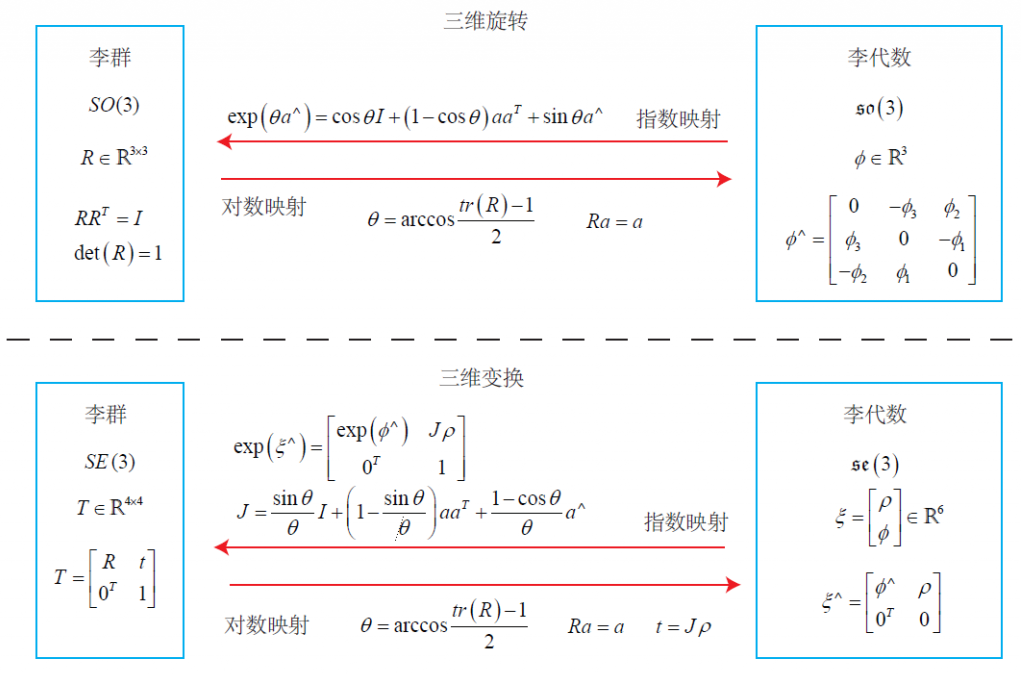
\includegraphics[height=9cm]{figures/lie.png}
\caption{SO(3),SE(3),$\mathfrak{so(3),se(3)}$的对应关系}
\end{figure}
\section{扰动模型}
接下来我们简单介绍一下SE(3)和SO(3)如何利用扰动模型求导。
\subsection{SO(3)上的扰动模型}
假设我们对一个空间点$\vec p$进行了旋转,得到了$\vec Rp$,那么要计算旋转之后的点的坐标相对于旋转的导数该如何计算呢?我们可以考虑对$\vec R$进行一个微小的扰动,也可以说是增量$\delta R$,假设这个扰动对应的李代数是$\varphi$,然后对$\varphi$求导,得:
\begin{equation}
\frac{\partial(\boldsymbol{R} \boldsymbol{p})}{\partial \boldsymbol{\varphi}}=\lim _{\varphi \rightarrow 0} \frac{\exp \left(\boldsymbol{\varphi}^{\wedge}\right) \exp \left(\boldsymbol{\phi}^{\wedge}\right) \boldsymbol{p}-\exp \left(\boldsymbol{\phi}^{\wedge}\right) \boldsymbol{p}}{\varphi}
\end{equation}
对小量进行泰勒展开,得:
\begin{equation}
\begin{aligned}
\frac{\partial(\boldsymbol{R p})}{\partial \varphi} &=\lim _{\varphi \rightarrow 0} \frac{\exp \left(\varphi^{\wedge}\right) \exp \left(\phi^{\wedge}\right) \boldsymbol{p}-\exp \left(\phi^{\wedge}\right) \boldsymbol{p}}{\varphi} \\ & \approx \lim _{\varphi \rightarrow 0} \frac{\left(1+\varphi^{\wedge}\right) \exp \left(\phi^{\wedge}\right) \boldsymbol{p}-\exp \left(\phi^{\wedge}\right) \boldsymbol{p}}{\varphi} \\ &=\lim _{\varphi \rightarrow 0} \frac{\varphi^{\wedge} \boldsymbol{R p}}{\varphi}=\lim _{\varphi \rightarrow 0} \frac{-(\boldsymbol{R p})^{\wedge} \varphi}{\varphi}=-(\boldsymbol{R p})^{\wedge}
\end{aligned}
\end{equation}
这里可能比较难以理解的是第三行,$\phi^\wedge\vec R \vec p$实际上等于$\phi\times (\vec R \vec p)$,根据叉乘的交换律,也就是$-(\vec R \vec p)\times \phi$,即:$-(\vec R \vec p)^\wedge \phi$。这个求导的结果是一个3$\times$3的矩阵,表示旋转后的三个维度,分别关于小扰动的三个分量的导数。
\subsection{SE(3)上的扰动模型}
同样的,假设我们对空间点$\vec p$进行了一次旋转+平移,得到了$\vec T p$\footnote{此处$\vec p$是齐次坐标。},现在,给T左乘一个扰动$\Delta T$=$\exp{(\delta \xi^\wedge)}$,设扰动的李代数$\delta \xi=[\delta \rho,\delta \phi]^T$,因此关于扰动的导数为:
\begin{equation}
\begin{aligned}
\frac{\partial(T p)}{\partial \delta \xi}
&=\lim _{\delta \xi \rightarrow 0} \frac{\exp \left(\delta \xi^{\wedge}\right) \exp \left(\xi^{\wedge}\right) p-\exp \left(\xi^{\wedge}\right) p}{\delta \xi} \\
& \approx \lim _{\delta \xi \rightarrow 0} \frac{\left(I+\delta \xi^{\wedge}\right) \exp \left(\xi^{\wedge}\right) p-\exp \left(\xi^{\wedge}\right) p}{\delta \xi} \\
&=\lim _{\delta \xi \rightarrow 0} \frac{\delta \xi^{\wedge} \exp \left(\xi^{\wedge}\right) p}{\delta \xi}\\
&=\lim _{\delta \xi \rightarrow 0} \frac{\left[ \begin{array}{cc}{\delta \phi^{\wedge}} & {\delta \rho} \\ {\mathbf{0}^{T}} & {0}\end{array}\right] \left[ \begin{array}{c}{\boldsymbol{R} p+t} \\ {\mathbf{1}}\end{array}\right]}{\delta \boldsymbol{\xi}}\\
&=\lim _{\delta \xi \rightarrow 0} \frac{\left[ \begin{array}{c}{\delta \phi^{\wedge}(R p+t)+\delta \rho} \\ {0}\end{array}\right]}{\delta \xi}=\left[ \begin{array}{cc}{I} & {-(R p+t)^{\wedge}} \\ {0^{T}} & {0^{T}}\end{array}\right] \triangleq(T p)^{\circ}
\end{aligned}
\end{equation}
$\circ$代表了将一个齐次坐标空间点变换成一个4$\times$6的矩阵。























